
\aaa{Singular Value Decomposition}

Let $A=\m1{0.5},01.$, the linear transformation of $A$ maps the circle of radius $1$ to an eclipse


\begin{tikzpicture}
    \draw[->] (-2,0) -- (2,0);
    \draw[->] (0,-2) -- (0,2);
    \draw[thick,red] (0,0) ellipse (1cm and 1cm);
\end{tikzpicture}
⟶  
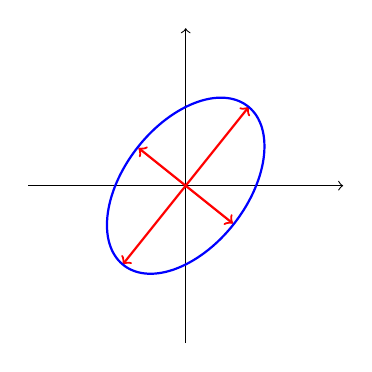
\begin{tikzpicture}
    \draw[->] (-2,0) -- (2,0);
    \draw[->] (0,-2) -- (0,2);
    \draw[red,thick,<->] (-0.8,-1.0)--(0.8,1.0);
    \draw[red,thick,<->] (-0.6,0.48)--(0.6,-0.48);
    \draw[thick,blue,cm={1,0.5,0,1,(0,0)}] (0,0) ellipse (1cm and 1cm);
\end{tikzpicture}

The singular value of $A$ is defined to be the length of the half-axes of eclipse after transformation. 
\a\aa
For this purpose, we consider a special case, if 
$$
A = Ω_1ΛΩ_2
$$
where $Ω_1^TΩ_1=I$;
$Ω_2^TΩ_2=I$;
$Λ$ a diagonal matrix.

\vfill

Applying the matrix $A$ is the same as applying three linear transformations.

\a\aa
First, applying Ω_2, it does not change the length of any vector, the circle stays as a circle.

\begin{tikzpicture}
    \draw[->] (-2,0) -- (2,0);
    \draw[->] (0,-2) -- (0,2);
    \draw[thick,red] (0,0) ellipse (1cm and 1cm);
\end{tikzpicture}
⟶  
\begin{tikzpicture}
    \draw[->] (-2,0) -- (2,0);
    \draw[->] (0,-2) -- (0,2);
    \draw[thick,red] (0,0) ellipse (1cm and 1cm);
\end{tikzpicture}
\a\aa
Second, applying the diagonal matrix, the circle would change only in the $x$ and $y$ direction

\begin{tikzpicture}
    \draw[->] (-2,0) -- (2,0);
    \draw[->] (0,-2) -- (0,2);
    \draw[thick,red] (0,0) ellipse (1cm and 1cm);
\end{tikzpicture}
⟶  
\begin{tikzpicture}
    \draw[->] (-2,0) -- (2,0);
    \draw[->] (0,-2) -- (0,2);
    \draw[thick,blue] (0,0) ellipse (1.3cm and 0.78cm);
\end{tikzpicture}
\a\aa
Finally, another rotation rotate the ellipse to another angle 
\begin{tikzpicture}
    \draw[->] (-2,0) -- (2,0);
    \draw[->] (0,-2) -- (0,2);
    \draw[thick,blue] (0,0) ellipse (1.3cm and 0.78cm);
\end{tikzpicture}
⟶
\begin{tikzpicture}
    \draw[->] (-2,0) -- (2,0);
    \draw[->] (0,-2) -- (0,2);
    \draw[thick,blue,cm={1,0.5,0,1,(0,0)}] (0,0) ellipse (1cm and 1cm);
\end{tikzpicture}
\a\aa
Therefore, in the form
$$
A = Ω_1ΛΩ_2,
$$
the diagonal matrix Λ exactly contains all the singular value of $A$.
\a\aa
Next, we claim that any matrix $A$ can be decomposed into the form
$$
A = Ω_1ΛΩ_2,
$$
so that we may read singular values of $A$ directly from $Λ$.
\a\aa
Method for decomposition. 

For $A= Ω_1ΛΩ_2$, we realize that
$$ A^TA = Ω_2^TΛΩ_1^TΩ_1ΛΩ_2 = Ω_2^TΛ^2Ω_2 $$
$$ AA^T = Ω_1ΛΩ_2Ω_2^TΛΩ_1^T = Ω_1^TΛ^2Ω_1 $$

\[rem]{For any matrix $A$, $A^TA$ and $AA^T$ are all positive semidefinite, therefore, all its eigenvalues are real and non-negative, and there exists orthogonal matirix Ω_2, but not unique, such that
$$
Ω_2 A^TA  Ω_2^T = \m{λ_1}{}{}{},{}{λ_2}{}{},{}{}\ddots{},{}{}{}{λ_n}.
$$
}
\a\aa
After finding Ω_2, our goal is to find Ω_1 and Λ such that
$$
AΩ_2^T = Ω_1Λ
$$
Now write
$$
Ω_2^T=\m{v_1}{v_2}{…}{v_n}. ␣  ⟹  
Ω_1Λ=\m{Av_1}{Av_2}{…}{Av_n}. 
$$
Note that $Av_i$ already orthogonal with $Av_j$ because
$$
(Av_i)^T(Av_j)= v_i^T A^TAv_j = λ_j v_i^Tv_j = 0.
$$
Recall that $v_1,…,v_n$ are all eigenvectors. We may rearrange them so that 
$v_1,…,v_m$ are eigenvectors of \x{non-zero eigenvalues}, and $v_{m+1},…,v_n$ are eigenvectors of \x{zero eigenvalues}.
\a\aa
So
$$
\m{Av_1}{Av_2}{…}{Av_m}{Av_{m+1}}{…}{Av_n}. 
$$
$$
= \m{Av_1}{Av_2}{…}{Av_m}0{…}0.
$$
Note that 
$$
(Av_i)^T(Av_i)=v_i^TA^TAv_i = λ_iv_i^Tv_i = λ_i
$$
Therefore, to obtain unit vector we do
$$
\m{\frac{Av_1}{\sqrt{λ_1}}}{\frac{Av_2}{\sqrt{λ_2}}}{…}{\frac{Av_m}{\sqrt{λ_m}}}0{…}0.
\m
{\sqrt{λ_1}}{}{}{}{}{}{},
{}{\sqrt{λ_2}}{}{}{}{}{},
{}{}{\ddots}{}{}{}{},
{}{}{}{\sqrt{λ_m}}{}{}{},
{}{}{}{}{0}{}{},
{}{}{}{}{}{\ddots}{},
{}{}{}{}{}{}0.
$$
\a\aa
Now we may complete this into a orthonormal basis 
$$
\m{\frac{Av_1}{\sqrt{λ_1}}}{\frac{Av_2}{\sqrt{λ_2}}}{…}{\frac{Av_m}{\sqrt{λ_m}}}{u_{m+1}}{…}{u_n}.
\m
{\sqrt{λ_1}}{}{}{}{}{}{},
{}{\sqrt{λ_2}}{}{}{}{}{},
{}{}{\ddots}{}{}{}{},
{}{}{}{\sqrt{λ_m}}{}{}{},
{}{}{}{}{0}{}{},
{}{}{}{}{}{\ddots}{},
{}{}{}{}{}{}0.
$$
Therefore, we find $Ω_2Λ$.

Therefore $AΩ_2^T=Ω_1Λ$ so $Ω_1^{T}AΩ_2^T = Λ$ and
$$
A = Ω_1ΛΩ_2
$$.

\a\aa
\exe Find a singluar value decomposition of 
$$
A=\m101,{-1}10.
$$
\sol We put 
$$
AA^T = \m2{-1},{-1}2.
$$
$$
“det“(tI-AA^T) = t^2 - 4t +3 = (t-1)(t-3).
$$
Note that $“det“(tI_m-AB)=t^{m-n}“det“(tI_n-BA)$, we have of course
$$
“det“(tI-A^TA)=t(t^2-4t+3) = t(t-1)(t-3)
$$
\a\aa
Find an eigenvector $v_3$ of eigenvalue $3$, calculate
$$
AA^T-I = \m1{-1},{-1}1.
$$
We have $v_3=\m1,{-1}.$

\vfill

Find an eigenvector $v_1$ of eigenvalue $1$, calculate

$$
AA^T-3I = \m{-1}{-1},{-1}{-1}.
$$
We have $v_1=\m1,1.$
\a\aa
To get eigenvector of $A^TA$, we automatically have eigenvectors of eigenvalue $1$ and $3$.
$$u_1= A^T v_1 = \m1{-1},01,10.\m1,1. = \m0,1,1.  $$
$$u_3= A^T v_3 = \m1{-1},01,10.\m1,{-1}. = \m2,{-1},1.  $$

\a\aa

$$
u_1u_1^T=\m000,011,011. \overset{“normalize“}{\underset{“to trace 1“}{⟶  }} \m000,0{\frac12}{\frac12},0{\frac12}{\frac12}.
$$

$$
u_3u_3^T=\m4{-2}2,{-2}1{-1},2{-1}1. \overset{“normalize“}{\underset{“to trace 1“}{⟶  }}  \m{\frac23}{-\frac13}{\frac13},{-\frac13}{\frac16}{-\frac16},{\frac13}{-\frac16}{\frac16}.
$$
Therefore, the third vector, an eigenvector of eigenvalue $0$ is given by
$$
\m{\frac13},{\frac13},{-\frac13}.  ␣   “We can take“ \m 1,1,{-1}.
$$
\a\aa
Here is the collection of orthogonal vectors
$$
\m021,
1{-1}1,
11{-1}.␣
$$

\a\aa
Therefore
$$
A^T
\m
{\frac{v_1}{||v_1||}}
{\frac{v_2}{||v_2||}}.
=
\m
{\frac{u_1}{||u_1||}}
{\frac{u_2}{||u_2||}}
{\frac{u_3}{||u_3||}}.
Λ
$$
We know that $Λ$ are diagonal matrix of squareroot of eigenvalues. We have
$$
Λ=\m1{0},{0}{\sqrt{3}},00.
$$
\a\aa
We have
$$
\m1{-1},01,10. 
\m
{\frac1{\sqrt2}}
{\frac1{\sqrt2}},
{\frac1{\sqrt2}}
{-\frac1{\sqrt2}}.
= 
\m
{0}{\frac2{\sqrt{6}}}{\frac1{\sqrt{3}}},
{\frac1{\sqrt2}}{-\frac{1}{\sqrt{6}}}{\frac1{\sqrt{3}}},
{\frac1{\sqrt2}}{\frac1{\sqrt{6}}}{-\frac1{\sqrt{3}}}.\m1{0},{0}{\sqrt{3}},00.
$$

Singular value decomposition
$$
\m1{-1},01,10. = 
\m
{0}{\frac2{\sqrt{6}}}{\frac1{\sqrt{3}}},
{\frac1{\sqrt2}}{-\frac{1}{\sqrt{6}}}{\frac1{\sqrt{3}}},
{\frac1{\sqrt2}}{\frac1{\sqrt{6}}}{-\frac1{\sqrt{3}}}.\m1{0},{0}{\sqrt{3}},00.
\m
{\frac1{\sqrt2}}
{\frac1{\sqrt2}},
{\frac1{\sqrt2}}
{-\frac1{\sqrt2}}.$$
\a\aa
Take transpose, we have singular value decomposition
$$
\m101,
{-1}10.
=
\m
{\frac1{\sqrt2}}
{\frac1{\sqrt2}},
{\frac1{\sqrt2}}
{-\frac1{\sqrt2}}.
\m100,0{\sqrt3}0.
\m
{0}{\frac1{\sqrt2}}{\frac1{\sqrt2}},
  {\frac2{\sqrt{6}}}{-\frac{1}{\sqrt{6}}}{\frac1{\sqrt{6}}},
  {\frac1{\sqrt{3}}}
{\frac1{\sqrt{3}}}
{-\frac1{\sqrt{3}}}..
$$
\aaa
